\chapter{Robot Dynamics Framework}
\label{sec:robotdynamic}

In this appendix, the nomenclature and the mathematical equations, used to represent the behavior of robotic systems in thesis, are presented. Table \ref{tab:nom} define all the variables.

\begin{table}[htbp]
	\centering
	\caption{Nomenclature}	% Table caption must be placed on top of the table %
		\begin{tabular}{ c c l r }
        \hline \hline
				\multicolumn{4}{c}{Scalars} \\
				\hline \hline
			$n$             &  :  & number of DoF                                              & \\
			$m$             &  :  & number of actuators                                        & \\
			$c$             &  :  & number of contact constraints                              & \\
			$o$             &  :  & number of end-effector coordinates                         & \\ 
			$l$             &  :  & number of discrete operating modes                         & \\ 
			$i$             &  :  & index for DoF                                              & \\
			$k$             &  :  & index for the operating mode                               & \\ 
			\hline \hline
			\multicolumn{4}{c}{Vectors} \\
			\hline \hline
			$\vec{\tau}$    &  :  & Electromagnetic motor torques                              & $m$  \\
			$\vec{q}$       &  :  & Joint coordinates position vector                          & $n$  \\
			$\vec{x}$       &  :  & Dynamic state vector $[\vec{\dot{q}} ;\vec{q}]$            & $2n$  \\
			$\vec{w}$       &  :  & Motor coordinates velocity vector                          & $m$  \\ 
			$\vec{g}$       &  :  & Gravitational forces vector                                & $n$  \\
			$\vec{c}$       &  :  & Sum of state-dependent generalized forces                  & $n$  \\
			$\vec{d}$       &  :  & Unknown disturbance forces                                 & $n$  \\
			$\vec{\tau}_I$  &  :  & Sum of intrinsic actuator forces                           & $m$  \\
			$\vec{\tau}_E$  &  :  & Sum of extrinsic forces                                    & $n$  \\
			$\vec{a}$       &  :  & Actuator coordinates position vector                       & $m$  \\
			$\vec{\phi}$    &  :  & Constraint vector                                          & $c$  \\
			$\vec{f}_c$     &  :  & Contact forces vector                                      & $c$  \\
			$\vec{f}_e$     &  :  & End-effector forces vector                                 & $o$  \\
			$\vec{p}$       &  :  & End-effector position vector                               & $o$  \\
			%$\vec{\lambda}$ &  :  & Coordinates of velocity subspace respecting constraints    & $n-c$  \\
			\hline \hline
			\multicolumn{4}{c}{Matrices} \\
			\hline \hline
			$H$             &  :  & Inertia matrix                                             & $n$ x $n$ \\
			$D$             &  :  & Damping matrix                                             & $n$ x $n$ \\
			$C$             &  :  & Coriolis/Centrifugal forces matrix                         & $n$ x $n$ \\
			$B$             &  :  & Motor torques / generalized forces matrix                  & $n$ x $m$ \\
			$R$             &  :  & Gear-ratio matrix                                          & $m$ x $m$ \\
			$I$             &  :  & Intrinsic actuator inertia matrix (diagonal)               & $m$ x $m$ \\
			$B$             &  :  & Intrinsic actuator damping matrix (diagonal)               & $m$ x $m$ \\
			$J_a$           &  :  & actuator coordinates / joint coordinates Jacobian matrix   & $m$ x $n$ \\
			$J_e$           &  :  & task-space coordinates / joint coordinates Jacobian matrix & $o$ x $n$ \\
			$J_c$           &  :  & Contact constraints Jacobian matrix                        & $c$ x $n$ \\ 
			%$V$             &  :  & Vector base of the velocity subspace matrix                & $n$ x $(n-c)$ \\ 
		\hline \hline
        \end{tabular}		
	\label{tab:nom}
\end{table}

\section{Equations of motions}
\label{sec:eom}

The general form of the equations of motion of robotic systems (interconnected rigid body driven by actuators) is:
%
\begin{align}
H(\vec{q}) \vec{\ddot{q}} + C(\vec{q},\vec{\dot{q}}) \vec{\dot{q}} + D \vec{\dot{q}} + \vec{g}(\vec{q}) = B(\vec{q}) \vec{\tau} 
\label{eq:manipulator}
\end{align}
%
where $\vec{q}$ is the generalized coordinates vector, $H$ is the inertia matrix, $C$ is the Coriolis/centrifugal force matrix, $D$ is a damping matrix, $\vec{g}$ is the gravitational forces vector and $B$ is a matrix mapping motor torques $\vec{\tau}$ into generalized forces.
%%
%Kinetic energy is given by:
%%
%\begin{align}
%\frac{1}{2} \vec{\dot{q}}^T H(\vec{q}) \vec{\dot{q}} 
%\label{eq:kinetic}
%\end{align}
%%
%Conservation of energy also give the following relation:
%%
%\begin{align}
%\dot{H} = C + C^T
%\label{eq:cener}
%\end{align}
%%
On occasion, dependence notation is dropped and $\vec{c}$ is used to represent all state dependent forces, leading to the short form:
%
\begin{align}
H \vec{\ddot{q}} + \vec{c} = B \vec{\tau} 
\label{eq:manipulator_short}
\end{align}

\section{Coordinate systems}
\label{sec:coord}

Fig. \ref{fig:coord} shows all the used coordinates systems. 
%
\begin{figure}[t]
	\centering
		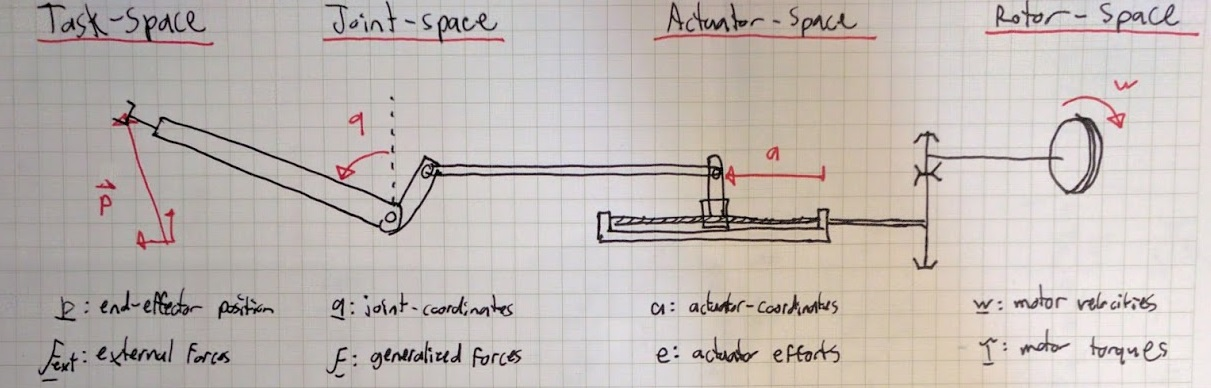
\includegraphics[width=0.99\textwidth]{coord.jpg}
	\caption{Coordinate systems}
	\label{fig:coord}
\end{figure}
%
The following equation represents the most general case:
%
\begin{align}
H_k \vec{\ddot{q}} + C_k \vec{\dot{q}} + D_k \vec{\dot{q}} + \vec{g} =  \underbrace{ J_a^T(\vec{q}) R^T }_{B(\vec{q})}  \vec{\tau} + J_e^T(\vec{q}) \vec{f}_e + J_c^T(\vec{q}) \vec{f}_c
\label{eq:manipulator_gen}
\end{align}
%
Where matrices with subscript $k$ include the motor-rotor dynamics contributions when the gear-ratio configuration $R_k$ is used:
%
\begin{align}
H_k   &= H + J_a^T R_k^T I_a R_k J_a        \\
C_k   &= C + J_a^T R_k^T I_a R_k \dot{J}_a \quad \text{if $R$ and $J_a$ are diagonal} \\
D_k   &= D + J_a^T R_k^T B_a R_k J_a 
\label{eq:coord_transform}
\end{align}
%
Coordinates transforms are defined by:
%
\begin{align}
\vec{\dot{p}}   &= J_e( \vec{q} ) \vec{\dot{q} }  \quad \text{ from joint-space to end-effector   } \\
\vec{\dot{a}}   &= J_a( \vec{q} ) \vec{\dot{q} }  \quad \text{ from joint-space to actuator-space } \\
\vec{w }        &= R              \vec{\dot{a} }  \quad \text{ from actuator-space to rotor-space } 
\label{eq:coord_transform2}
\end{align}
%
Note that the distinction between actuator output coordinates and joint coordinates, useful for the DSDM-Arm shoulder mechanism, is omitted for brevity in Chapter \ref{sec:ControlAndPlanningOfRobotUsingVariableGearRatioActuators}. 

\section{Contact}
\label{sec:contact}

This section presents equations for representing contact situations.

\subsection{Kinematic constraints}
\label{sec:constraints}
%
If a robotic manipulator enter contact with a fixed object, then some DoF are constrained. In the case of a bilateral constraint, the constraint can be expressed as:
\begin{align}
\vec{\phi}( \vec{ q } ) = 0
\label{eq:constraint}
\end{align}
%
The time-derivative of the constraint must also be equal to zero, which gives some constraints in terms of velocity and acceleration:
\begin{align}
\frac{d \vec{\phi}( \vec{ q } ) }{dt}     &= J_c( \vec{ q } ) \vec{\dot{q}}  = 0 \\
\frac{d^2 \vec{\phi}( \vec{ q } ) }{dt^2} &= J_c( \vec{ q } ) \vec{\ddot{q}}  + \dot{J}_c( \vec{ q } ) \vec{\dot{q}} = 0 
\label{eq:constraint_diff}
\end{align}
%
when $J_c$ is the constraint Jacobian:
%
\begin{align}
J_c( \vec{ q } )                    &= \frac{d \vec{\phi}( \vec{ q } ) }{d\vec{ q }}
\label{eq:constraint_jaco}
\end{align}

\subsection{Constraint forces}
\label{sec:constraint_forces}

The constraint Jacobian can be used to map constraint forces $\vec{f}_c$ to generalized forces in the EoM:
%
\begin{align}
H \vec{\ddot{q}} + \vec{c} = B \vec{\tau} + J_c( \vec{ q } )^T  \vec{f}_c
\label{eq:manipulator_constraint}
\end{align}
%
Solving for $\vec{\ddot{q}}$ in eq. \eqref{eq:manipulator_constraint} and substituting in eq. \eqref{eq:constraint_diff}, it is possible to get and expression for the constraint forces $\vec{f}_c$ as a function of states and applied torques:
%
\begin{align}
\vec{f}_c = \left( J_c H^{-1} J_c^T \right)^{-1} \left(  J_c H^{-1} [\vec{c} - B \vec{\tau} ] - \dot{J}_c( \vec{ q } ) \vec{\dot{q}}   \right)
\label{eq:const_forces}
\end{align}
%
Alternatively, it possible to solve for acceleration $\vec{\ddot{q}}$ and constraints forces $\vec{f}_c$ simultaneously by solving the following system of equations:
%
\begin{align}
\left[ \begin{array}{c c } 	H & -J_c^T  \\ J_c 	& 0  	\end{array} \right] \left[ \begin{array}{c} \vec{\ddot{q}}  \\ \vec{f}_c \end{array} \right] = \left[ \begin{array}{c}  B \vec{\tau} - \vec{c}   \\ -\dot{J}_c \vec{\dot{q}}  \end{array} \right]
\label{eq:manipulator_constraint_eom}
\end{align}


\subsection{Impact impulsive behavior}
\label{sec:impact}
%
When the robot first enters contact with a fixed object, impulsive contact forces will act on the system. Integrating eq. \eqref{eq:manipulator_constraint} over the short impact interval gives:
%
\begin{align}
\int{ ( H \vec{\ddot{q}} + \vec{c} ) dt } &= \int{ ( B \vec{\tau} + J_c( \vec{ q } )^T  \vec{f}_c ) dt } \\
H \vec{\dot{q}}^+ - H \vec{\dot{q}}^- &= J_c( \vec{ q } )^T  \int{  \vec{f}_c dt }
\label{eq:manipulator_impact}
\end{align}
%
where any non-impulsive forces are neglected during the short impact interval. Projecting onto constrained coordinates (multiplying by $J_c H^{-1}$) gives:
%
\begin{align}
J_c \vec{\dot{q}}^+ - J_c \vec{\dot{q}}^- &= J_c H^{-1} J_c^T  \int{  \vec{f}_c dt }
\label{eq:manipulator_impact2}
\end{align}
%
Then assuming a sticky inelastic impact (no bouncing), then the constraint is respected after the impact ($J_c \vec{\dot{q}}^+=0$) and it is possible to solve for the impact force:
%
\begin{align}
\int{  \vec{f}_c dt } &= - \left( J_c H^{-1} J_c^T \right)^{-1}  J_c \vec{\dot{q}}^-
\label{eq:manipulator_impact_force}
\end{align}
%
and also for the velocity after the impact:
%
\begin{align}
\vec{\dot{q}}^+ &= - \Big[ I - H^{-1} J_c^T \left( J_c H^{-1} J_c^T \right)^{-1} J_c \Big] \vec{\dot{q}}^-
\label{eq:manipulator_impact_velocity}
\end{align}
%
Or change in velocity:
%
\begin{align}
\Delta \vec{\dot{q}} &=  \Big[ H^{-1} J_c^T \left( J_c H^{-1} J_c^T \right)^{-1} J_c \Big] \vec{\dot{q}}^-
\label{eq:manipulator_impact_velocity_delta}
\end{align}
%

Alternatively, it possible to solve for velocity $\vec{\dot{q}}^+$ and impulsive forces $\int{ \vec{f}_c dt }$ simultaneously by solving the following system of $n+c$ equations:
%
\begin{align}
\left[ \begin{array}{c c } 	H & -J_c^T  \\ J_c 	& 0  	\end{array} \right] \left[ \begin{array}{c} \vec{\dot{q}}^+  \\ \int{ \vec{f}_c dt }\end{array} \right] = \left[ \begin{array}{c}  	H \vec{\dot{q}}^-   \\ 0  \end{array} \right]
\label{eq:manipulator_impact_eom}
\end{align}


%Instead of augmenting the system with constraint equations,  it is also possible to parametrize the subspace of velocities that satisfy the contact constraint (which correspond to the nullspace of $J_c$):
%%
%\begin{align}
%\vec{\dot{q}}^+ &= V \vec{\lambda} = \vec{v}_1 \lambda_1  + ... + \vec{v}_{n-l} \lambda_{n-l} \\
%& \quad \text{with} \quad J_c V \vec{\lambda} = 0 \quad \forall \quad \vec{\lambda} \in \Re^{n-l}
%\end{align}
%%
%and solve the following smaller system of $n$ equations:
%%
%\begin{align}
%\Bigg[ \begin{array}{c c } 	H V & -J_c^T  	\end{array} \Bigg] \left[ \begin{array}{c} \vec{\lambda}  \\ \int{ \vec{f}_c dt }\end{array} \right] = H \vec{\dot{q}}^-
%\label{eq:manipulator_impact_eom}
%\end{align}


\section{Hybrid system dynamics}

Hybrid dynamical system can be represented in the general form:
%
\begin{align}
\text{Continuous evolution: } \left(  \dot{\vec{x}} , \dot{k} \right) &=  \left( \, f_k( \vec{x} , \vec{u} , \vec{d} ) \, , \, 0 \, \right) \\
\text{Discrete jumps: } \left(  \vec{x}^+ , k^+ \right) &=  \left( h_{ij}( \vec{x}^- , \vec{u}^- ) , j \right) \quad\text{if}\quad \left(  \vec{x} , k , \vec{u} \right) \in D_{ij}  
\end{align}
%
where $\vec{x}$ is a continuous state vector, and $k$ is a discrete mode and $D_{ij}$ is the domain mapping conditions leading to a transition $k:i \rightarrow j$. For robotic systems, the discrete mode can represent discrete configurations of the robot , like gear-ratios in this thesis, and contact/non-contact conditions. The jump map then represents the impulsive response when contact is made. 

\subsection{Switched system}

A restricted class of hybrid system, called switched system, are hybrid systems for which the jump map for continuous state is the identify function:
%
\begin{align}
\text{Continuous evolution: } \left(  \dot{\vec{x}} , \dot{k} \right) &=  \left( \, f_k( \vec{x} , \vec{u} , \vec{d} ) \, , \, 0 \, \right) \\
\text{Discrete jumps: } \left(  \vec{x}^+ , k^+ \right) &=  \left( \vec{x}^- , j \right) \quad\text{if}\quad \left(  \vec{x} , k , \vec{u} \right) \in D_{ij} 
\end{align}
%

\subsubsection{Switched system where the discrete mode is a control input}

In the situation where the discrete operating mode $k$ is a control input, then there is no need to keep track of discrete mode evolution and only the piece-wise continuous differential equations are sufficient to model the system evolution:
%
\begin{align}
\dot{\vec{x}} = f_k( \vec{x} , \vec{u} , \vec{d} ) 
\end{align}
%
The model for robots using variable transmissions with discrete configurations, that is used in Chapter \ref{sec:ControlAndPlanningOfRobotUsingVariableGearRatioActuators}, is of this category. 
